\documentclass[10pt,a4paper]{article}
\linespread{1.5}

\usepackage{float}
\usepackage[T1]{fontenc}
\usepackage{amsfonts}
\usepackage[utf8]{inputenc}
\usepackage{graphicx}
\usepackage{url} % príkaz \url na formátovanie URL
\usepackage{hyperref} % odkazy v texte budú aktívne (pri niektorých triedach dokumentov spôsobuje posun textu)
\setlength{\parindent}{0pt}
\newcommand{\parindentplus}{\hspace*{\parindent}\vspace{0em}}
\usepackage{cite}
\usepackage{multirow}

\pagestyle{headings}

\title{Ensuring Data Integrity and Reliability in Big Data\thanks{Semestrálny projekt v predmete Metódy inžinierskej práce, ak. rok 2023/24, vedenie: Mirwais Ahmadzai}}

\author{Michal Zrutta \\[2pt]
	{\small Slovenská technická univerzita v Bratislave}\\
	{\small Fakulta informatiky a informačných technológií}\\
	{\small \texttt{xzrutta@stuba.sk}}
}
\date{\small 5. November 2023}
\begin{document}

\maketitle



\begin{abstract}

We live in the era of Big Data.These days data comes too fast and in an enormous sizes, this requires better understanding of data and processing. Data generation increased by 95 zettabytes between 2010 and 2022.\\However, the upward trajectory poses challenges in data quality. Consequently, the demand for realistic data sets, accurate and consistent information, and overall data quality has become a pressing concern.\\This study delves into the challenges of data quality assurance in the realm of Big Data analytic, exploring methodologies to validate diverse and extensive data-sets. The research is shown on a context of car gas consumption model.\\The paper later shows potential but already used integration of Artificial Intelligence. AI algorithms are supposed to identify and rectify inaccuracies, while also learning from the data to continuously enhance data quality.
\end{abstract}



\section{Introduction}

\subsection{Background}

In recent times, the term "Big Data" has become widespread, describing a massive amount of information flooding businesses, organizations, and research institutions daily. Big Data includes data-sets that are too large, complex, or fast-moving for regular data processing tools.\cite{mittal2013trustworthiness} Data comes from various sources like social media, sensors, online transactions, and multimedia. What makes Big Data unique isn't just its enormous size but also its speed, diversity, and reliability.\cite{gudivada2015big}
The rapid growth and widespread use of Big Data technologies have transformed industries and research fields globally. With the increasing digitization of information and advancements in data processing capabilities, organizations now have the ability to collect, store, and analyze massive volumes of data in real-time. This growth has been driven by the need to extract valuable insights, improve decision-making processes, enhance customer experiences, and gain competitive advantages.\cite{fanelli2023big} Industries ranging from business and health-care to science and social sciences have embraced Big Data technologies, leading to their everywhere use in diverse applications.\cite{anisetti2023assurance}
This requires accurate and precise data analysis to extract valuable insights, ensuring its usefulness across a wide range of industries. Trustworthiness in dealing with Big Data is really important. It means the information used is reliable and accurate, preventing mistakes. It also builds people's confidence and protects their privacy in our data-driven world.\cite{anisetti2023assurance}
\paragraph{History.}
The history of Big Data can be tracked back to the late 1970s when the concept of the "database machine". As the volume grew, the limitations of single mainframe systems led to proposal of a "share nothing". It is a parallel database system that met demand of increasing data volume. The Teradata system marked a milestone in 1986.\cite{chen2014big}  Challenges arose with the rise of Internet services, leading to the development of GFS and MapReduce by Google. In 2011, EMC/IDC's research report introduced big data's concept and potential. Major companies like Oracle, Microsoft, Google, Amazon, and Facebook, initiated big data projects.\cite{chen2014big} The economic significance of big data was underscored in 2012, likening it to a new kind of economic asset.
\cite{chen2014big} 

\subsection{Problem Statement}

Big data analysis can transform raw data collected from users in a big data program into useful information. Wrong data and incorrect inputs can significantly alter the overall results, which are crucial in many cases.\cite{8063921} Having too much unnecessary and repeating data can make predictions less accurate and cause mistakes in decision-making. This can lead to unexpected losses and risks.\cite{10165495} Having high-quality data can enhance the potential for delivering excellent services within an organization.\cite{6204995} While existing literature addresses concerns about data reliability, the question persists: How can we ensure data quality?

\section{Previous Studies on Data Quality in Big Data}

\subsection{Data Accuracy and Reliability for Big Data}
In the proposed data quality assessment process for big data, as outlined by Li Cai from Yunnan University, the initial step involves defining data collection goals aligned with strategic objectives. Users choose data based on factors like operations, decision-making, and planning. Quality elements vary with business environments; for example, social media data prioritize timeliness and credibility.\cite{article}
Specific dimensions, indicators, and assessment criteria are determined for each business context. Data cleaning is crucial for error detection and removal, enhancing data quality. The data acquisition phase employs various methods such as integration, search-download, and web crawlers.\cite{article}

\newpage

\begin{figure*}[htbp]
  \centering
  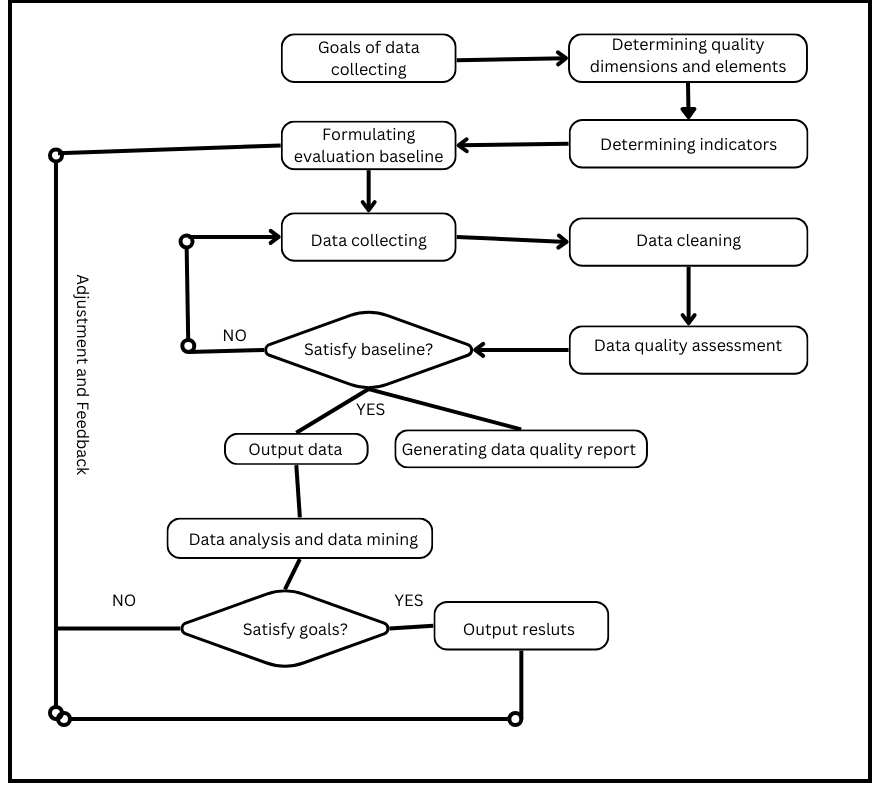
\includegraphics[width=0.8\columnwidth]{Quality assesment process for Big Data.png}
  \caption{Quality assessment for big data}
  \label{fig:quality-assessment}
\end{figure*}

Following data collection, the paper emphasizes the importance of data cleaning to address issues like errors and inconsistencies. The assessment then enters qualitative and quantitative evaluation phases. If data quality meets the baseline standards, analysis proceeds, generating quality reports. Otherwise, adjustments are made, and new data acquisition may be necessary.\cite{article}
\\
While data analysis and mining aren't directly part of quality assessment, they play a vital role in dynamic adjustment and feedback. Successful analyses feed back into the quality assessment system, supporting continuous improvement. Adjustments are made if analysis results don't align with goals, ensuring an iterative and adaptive data quality assessment process.\cite{article}

\subsection{Semantic Integrity Analysis for Unstructured Big Data}
This study is dedicated to the evaluation of unstructured Big Data, focusing on a assessment process for unstructured datasets. The model show us several essential components that collectively contribute to the comprehensive evaluation of data quality, resulting in a detailed quality assessment report.\cite{8605945}

\begin{enumerate}
\item \textbf{Quality Requirements:} The process initiates with defining precise quality requirements aligned with the strategic objectives, ensuring that the assessment is tailored to meet specific business goals.
\item \textbf{Data Sources:} Unstructured data is diverse and originates from varied sources. Evaluating its quality necessitates a clear understanding of these sources, encompassing social media, sensors, multimedia, and other channels.
\item \textbf{Data Quality Repository:} A centralized repository is established to store and manage data quality-related information, facilitating seamless tracking and analysis.
\item \textbf{Sampling and Profiling:} The data undergoes sampling and profiling, enabling a deeper understanding of its characteristics and patterns, which is fundamental for quality evaluation.
\item \textbf{Preparation Process for Quality Evaluation:} Preparing the data for evaluation involves preprocessing steps to ensure consistency and completeness, laying the foundation for accurate assessment.
\item \textbf{Feature Selection and Quality Mapping:} Relevant features are meticulously selected, and quality mapping techniques are applied, allowing for a focused evaluation process and ensuring that quality assessment aligns with the specific attributes of unstructured data.
\item \textbf{Quality Assessment:} Utilizing both qualitative and quantitative methods, the data undergoes a rigorous evaluation. Qualitative analysis conducted by experts evaluates data based on specific criteria, while quantitative methods provide objective insights.
\end{enumerate}
\cite{8605945}

\subsection{AI and Crowdsourcing Solutions}

Various studies demonstrate how AI can assist in managing Big Data lakes and handling diverse data from various sources, addressing challenges such as incomplete data, invalid entries, and uncertainties.
AI and crowsdsourcing can be used in this problem. AI is able to remove duplicates from database or knowledge base. And there are continuous studies in data quality.\cite{6949519}
\\
In another study they've come out with PClean. PClean is a system developed by MIT researchers that automatically cleans "dirty data" by addressing issues such as typos, duplicates, missing values, misspellings, and inconsistencies.\cite{lew2021pclean}
PClean is designed to automate the data cleaning process, reducing the time and effort required by data analysts, engineers, and scientists. It is efficient in terms of both accuracy and runtime. It outperforms benchmarks with just 50 lines of code, making it a more streamlined solution compared to alternative state-of-the-art options. \cite{lew2021pclean}
\paragraph{Sustainability and Ethics.}
Sustainability is really important when it comes to protection of hardware or use of electricity. We could see power cut of university cloud at the start of semester due to hardware collision. When the code is reduced it means it is more effective and also efficient which results in protecting hardware. What is more, efficient coding and data storage techniques not only enhance data quality but also contribute to a more sustainable use of computing resources, reducing energy consumption. The use of renewable energy, such as solar power, supports sustainability in powering data centers. Respecting user privacy and asking his permission to collect important data contribute to a sustainable and responsible approach to data management.


\section{Methodology}
In crafting the methodology for this article, a comprehensive examination of existing literature and research on the subject of ensuring data quality served as the foundation. Different perspectives and approaches from various articles and studies paved the way for the innovation of a novel approach to address the obstacles of data quality in the background of Big Data.\cite{ji2020quality} The key steps of the developed methodology are outlined below:

\begin{enumerate}
    \item \textbf Literature Review
    \item \textbf Understanding the problem
    \item \textbf Identification of similar approaches
    \item \textbf Innovation through Integration
    \item \textbf Validation through a hierarchical data quality standard
\end{enumerate}

Through the systematic execution of these steps, the resulting methodology not only builds upon the wealth of existing knowledge but also introduces a fresh perspective that is responsive to the evolving landscape of Big Data.
 

\subsection{Proposed Methodology for Data Quality Assurance in Big Data}

If we had to collect data from all specific car model in the world for particular information, for example gas consumption.
Firstly we would need to specify:

\begin{enumerate}
    \item \textbf{Where?} It is really important where the car is driven. If it is somewhere rainy, for example Britain, or in Australia where it is hot, or in Canada where it is cold. The car and it's use is totally different and collected data which are not selected correctly would result in not proper product. For example electric cars like Tesla have difficulties in cold environment.
    \item \textbf{Who?} Everybody drives their cars differently so in order to get good results we need drivers who have similar driving skills.
    \item \textbf{When?} The time of data collection is crucial. Gas consumption can vary based on the time of day, traffic conditions, and seasons. For instance, in urban areas, gas consumption might differ during rush hours compared to non-peak times. Similarly, seasonal variations, such as summer and winter, can impact a car's fuel efficiency. Collecting data over different times and seasons can provide a comprehensive understanding of gas consumption patterns.
\end{enumerate}

Secondly, I recommend implementing a user ranking system for data contributors. Because if he is not qualified as a driver who has driving style as we need. For example, if a participant drives their car in a desert, which is vastly different from the study's target environments, their data might not be suitable for the overall analysis.\cite{8605945}
\\Once the data is collected from verified users we have to clean them and sort them out.
As you can see in previous study we can use AI to help us clear and clean data to enhance data accuracy. AI can automatically identify and correct mistakes. \\Additionally, AI possesses a deep understanding of physics, enabling it to perform calculations to validate the data accuracy and identify errors. \\Moreover, AI systems incorporate self-learning mechanisms, allowing them to learn from the collected data. This self-learning capability ensures continuous improvement in data quality over time by learning from past mistakes and refining its algorithms for future analyses.\cite{6949519}


\subsection{Quality Standards for Large Datasets}
This table serves as a guide for understanding aspects that contribute to the overall quality of data.

\newpage

\begin{table}[H]
\small % Adjust the font size if needed
\begin{tabular}{|l|l|l|}
\hline
Dimensions                                                     & Elements      & Indicators                                                                                                                                                                                                                                                         \\ \hline
\multirow{2}{*}{Availability}                                  & Accessibility & \begin{tabular}[c]{@{}l@{}}Data access interface provided\\Easily accessible for public use or purchase\end{tabular}                                                                                                                           \\ \cline{2-3} 
                                                               & Timeliness    & \begin{tabular}[c]{@{}l@{}}Data arrive within schedule\\ Data are regularly updated\\ The time from data collection\\ through processing to release satisfies criteria\end{tabular}                                   \\ \hline
Usability                                                      & Credibility   & \begin{tabular}[c]{@{}l@{}}Data are sourced from specialized organizations\\ Data are regularly audited and checked by experts\\ Data are within acceptable value range\end{tabular} \\ \hline
\multirow{4}{*}{Reliability}                                   & Accuracy      & \begin{tabular}[c]{@{}l@{}}Data are accurate\\ Data provided accurately represent\\ the true state of source information\end{tabular}                                             \\ \cline{2-3} 
                                                               & Consistency   & \begin{tabular}[c]{@{}l@{}}Concepts, value domains, and formats\\ remain unchanged after processing\\ Data are in a constant behaviour\end{tabular}                                                              \\ \cline{2-3} 
                                                               & Integrity     & \begin{tabular}[c]{@{}l@{}}Data meets criteria of clear format\\  Data are consistent with structural integrity\\ Data are consistent with content integrity\end{tabular}                                                                                   \\ \cline{2-3} 
                                                               & Completeness  & \begin{tabular}[c]{@{}l@{}}If a component is deficient,\\ it will affect the utilization of multi-component data\\ and compromise both data accuracy and integrity.\end{tabular}                                                \\ \hline
Relevance                                                      & Fitness       & \begin{tabular}[c]{@{}l@{}}Data may not fully match the theme,\\ but illuminate one aspect\\ Most retrieved data sets meet user needs\\ and match their retrieval theme\end{tabular}      \\ \hline
\begin{tabular}[c]{@{}l@{}}Presentation\\ Quality\end{tabular} & Readability   & \begin{tabular}[c]{@{}l@{}}Clear and understandable content, meets user needs,\\and keeps to specifications in description, classification,\\ and coding\end{tabular} \\ \hline
\end{tabular}
\caption{The hierarchical framework for evaluating big data quality.}
\end{table}

Each dimension represents a critical aspect of data quality, and within each dimension, various elements and indicators provide understanding of the criteria for assessing data reliability.\cite{article}

\section{Objectives}
This paper aims to explore strategies ensuring data quality within the realm of Big Data. By addressing the challenges associated with incorrect data and not verified data it proposes methodologies to validate data quality. Through these strategies, the paper seek to help sort and clean data for reliable, accurate, and trustworthy data analysis in the era of Big Data.

\section{Analysis}

In this section,  a data analysis is presented focusing on gas consumption data collected from a car driven by me, my sister, and my mother. I compare data collected during periods when only my mother was the driver with data from a period when all of us shared the same car. Additionally, I analyze the data to show differences in gas consumption when the car is driven in cold or hot temperatures.

\subsection{Average Consumption}

The average consumption of a car is a crucial factor for many individuals when making a purchase decision. Precision and trustworthiness in the collected data are primary considerations for such decisions. Table 2 below highlights the difference in average consumption. The first column comprises data collected over seven years when solely my mother drove the car, while the second column features data from the last four years when the car was shared among all family members.

\begin{table}[h]
  \centering
  \begin{tabular}{|c|c|}
    \hline
    \textbf{Driven by mother} & \textbf{Driven by everybody} \\
    \hline
    4.90 l/km & 5.60 l/km \\
    \hline
  \end{tabular}
  \caption{Comparison of Average Gas Consumption}
\end{table}

The observed difference in average consumption is noteworthy, impacting the overall cost of operating the vehicle. A higher average consumption may indicate increased fuel expenses, which can influence the long-term financial aspects of owning the car. Furthermore, it raises the possibility that my mother is a more skilled and efficient driver, as evidenced by her ability to drive more economically than both my sister and me combined.
\\
To better understand the variations, it is essential to delve into factors such as driving habits, maintenance practices, and the change from longer drives to short drives. These insights can contribute to a more informed analysis and aid in decision-making for potential car buyers.

\subsection{Influence of Temperature}

The cold start or heating of the car during cold winters is a crucial element in the upward trajectory of gas consumption.\cite{zhu2021effects} This difference in collected data and can change overall results. As shown in Figure 2, there are 6 groups. Blue column represent month fro October till March, and orange column represent April til September. It is visible that during cold winter there is higher gas consumption.\\It is important to consider that during winter, the car was used for shorter distances, resulting in higher gas consumption.

\begin{figure}[htbp]
  \centering
  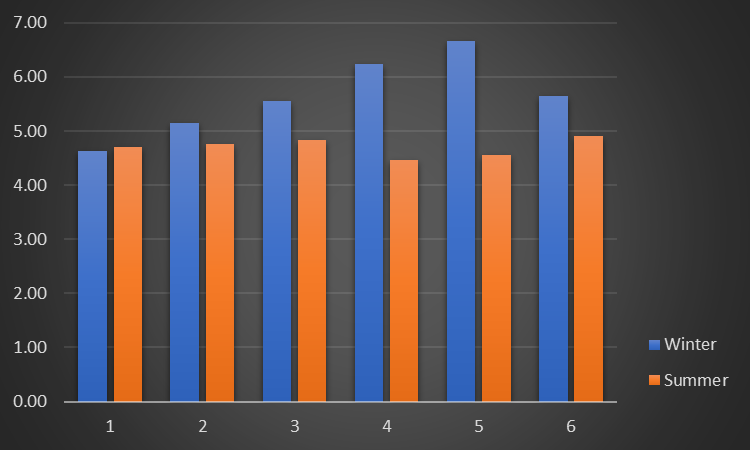
\includegraphics[width=1\linewidth]{Comparison.png}
  \caption{Comparison between winter and summer}
  \label{Figure 2}
\end{figure}

This visual representation provides a clear comparison between gas consumption in winter and summer months.



\section{Results}

In this section, we present a summary of the results obtained from the application of our proposed methodology for data quality assurance in the context of car gas consumption.

\subsection{Data Collection and Selection}

The data collection process focused on obtaining information about gas consumption in specific car model under varying conditions. Key aspects considered during data collection included geographical location, driver qualifications, and the timing of data collection.

\subsubsection{Geographical Considerations}

The geographical location of the data collection significantly influenced the results. For example, car driven in colder climates exhibited different gas consumption patterns compared to the car driven in warmer environments. This emphasizes the importance of considering the location factor in data selection.

\subsubsection{Driver Qualifications}

The user ranking system implemented for data contributors played a crucial role in ensuring the quality of the collected data. Drivers with similar driving styles were prioritized, leading to a more homogeneous data-set.

\subsubsection{Timing of Data Collection}

Variations in gas consumption based on the time of day, traffic conditions, and seasons were evident in the collected data. This highlights the importance of capturing data over different times and seasons to obtain a comprehensive understanding of gas consumption patterns.

\subsection{Data Cleaning and AI Integration}

Following data collection, the integration of artificial intelligence (AI) proved instrumental in enhancing data accuracy and reliability. The AI system automatically identified and corrected errors, leveraging its understanding of physics and self-learning mechanisms. This resulted in a more refined data-set suitable for analysis.



\section{Conclusion}

In conclusion, this article delves into the challenges and methodologies associated with ensuring data quality in the era of Big Data, with a specific focus on car gas consumption. The rapid increase of data in the past years has shown great challenges, in order to verify and improve the reliability of data.
\\
The proposed methodology include a comprehensive examination of existing literature, an understanding of the problem domain, identification of similar approaches, innovation through integration, and validation through a hierarchical data quality standard. By systematically executing these steps, the methodology aims to address the evolving landscape of Big Data and contribute to the field of data quality assurance.
\\
The analysis presented in this article compares gas consumption data under different driving conditions and explores the influence of temperature on the results. The findings highlights the importance of considering geographical factors, driver qualifications, and timing during data collection. Additionally, the integration of artificial intelligence proves beneficial in cleaning and refining the collected data, enhancing accuracy and reliability.
\\
The results obtained from the application of the proposed methodology highlight the impact of various factors on gas consumption, providing valuable insights for potential car buyers and contributing to the overall understanding of data quality in Big Data analytic.
\\
In summary, this article contributes to the ongoing lecture on data quality in the context of Big Data, offering a perspective and practical methodologies for ensuring reliability and accuracy in data analysis.

\paragraph{People and work: Scrum.}
From my own experience it is hard to lead people or a team even in the easiest tasks. I was not able to get three students working together on a group presentation. Here Scrum helps. Because we can divide project into smaller parts and assign it to co-workers. This not only allows for a more focused approach to work but also helps in better collaboration because each co-worker knows what his role is. The leader is responsible for his team and he needs to maintain and prioritize the backlog. It brings clarity to project priorities. It ensures that the team is working on tasks that are related to project and with targeted goals. We have sprint planning which helps in productivity. It is important to mention that communication, collaboration and commitment from all team members is crucial factor in getting the work done.
\\
\paragraph{Bachelor.}
In my opinion, a bachelor's degree signifies a comprehensive achievement.  In the field of IT it means that I should possess professional knowledge, soft skills, teamwork, procedures and techniques, programming skills, problem solving, critical thinking, . This indicates that people who has a degree in IT should be able to find a job in IT. Companies more likely prefer students with a degree than person who did not get through "hard" years of studying. Bachelor or higher education can secure me a better salary and place.

\bibliographystyle{abbrv}
\bibliography{citations}
\end{document}